\subsection{Problema a resolver}

El siguiente ejercicio se da en el contexto de un museo donde se requiere, por cuestiones de seguridad, colocar sensores de forma tal que todo el piso esté cubierto por los lásers que estos emiten. Existen dos tipos de sensores: los bidireccionales (que emiten señales horizontales o verticales) y los cuatridireccionales (que emiten señales verticales y horizontales). Los precios de éstos son \$4000 y \$6000 respectivamente. Se pide, también, que un sensor no apunte hacia otro dado que esto podría dejarlos sin funcionar. Además, se pide que ciertos lugares, definidos como \textit{importantes}, sean atravesados por dos lásers simultáneamente. El objetivo del algoritmo a realizar consiste en encontrar una forma de colocar los sensores de manera que el suelo quede completamente cubierto y que los lugares \textit{importantes} estén atravesados por un láser horizontal y otro vertical utilizando el mínimo costo posible. Por otra parte, debe ser tenido en cuenta que el museo cuenta con paredes que pueden interferir los lásers de los sensores.\newline

\newline
\textbf {Formatos de entrada y salida:}\newline
\newline
La entrada del algoritmo contiene una instancia del problema. La primera línea indica las dimensiones $n$ y $m$ de la grilla. A esta línea le siguen $n$ líneas, cada una con $m$ valores separados por espacios, indicando el contenido de cada una de las $n$ x $m$ casillas de la grilla, donde un 0 representa una pared, un 1 representa un casillero libre común y un 2 representa un casillero libre importante.\newline

En el caso en el que el problema no tenga solución, la salida deberá contener únicamente una línea con el valor -1. Caso contrario, la salida debe comenzar con dos números enteros: 
$$S\ C$$ 
donde $S$ es la cantidad de sensores utilizados y $C$ es el costo total de la solución. Luego, para cada sensor utilizado, debe haber una línea con el siguiente formato: 
$$t\ f\ c$$ 
donde $t$ es el tipo de sensor y $(f,c)$ son la fila y columna en donde éste se ubica (la esquina superior izquierda de la grilla es la posición (1,1) y la inferior derecha es la $(n,m)$). Para los sensores cuatridireccionales, $t$ debe valer 1, para los bidireccionales en forma horizontal $t$ debe valer 2 y en forma vertical 3.\newline
\newline
Dos ejemplos de este problema son los siguientes:

\begin{itemize}
\item {\large{\textbf{Ejemplo 1:}}}

\begin{figure}[H] % indico que voy a poner una figura y [h] indica que la posición relativa, tambien puedo usar t = top entre otros.
\hfill
\begin{minipage}[t]{.45\textwidth}
\begin{center}
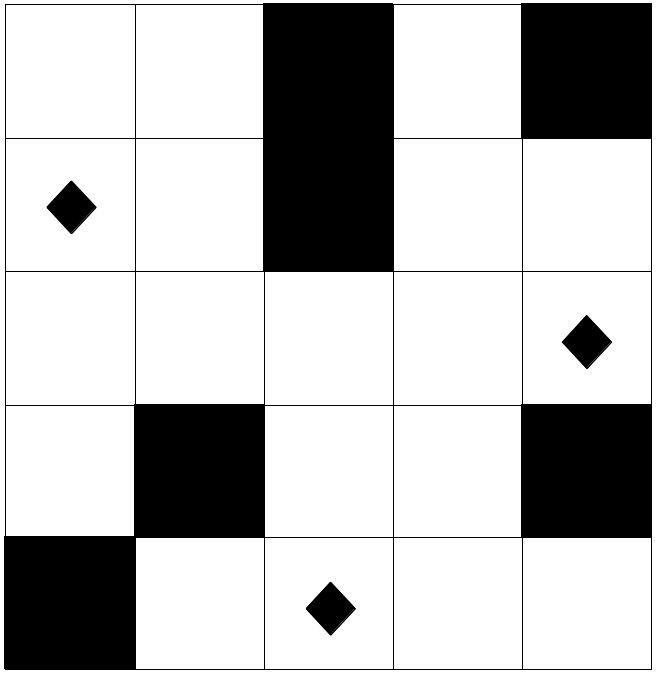
\epsfig{file=ejemplo1_ej3.jpg, scale=0.15} % primera imagen colocada a la izquierda
\caption{Ejemplo de la entrada de un caso con solución.}
\label{fig-tc1}
\end{center}
\end{minipage}
\hfill
\begin{minipage}[t]{.45\textwidth}
\begin{center}
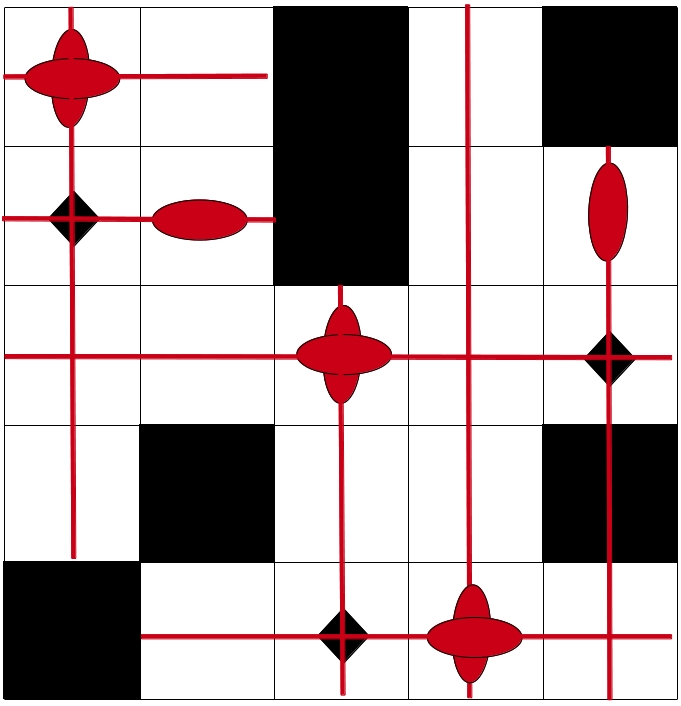
\epsfig{file=solucion_ejemplo1_ej3.jpg, scale=0.15} % segunda imagen colocada a la derecha
\caption{Ejemplo de la salida de un caso con solución.}
\label{fig-tc2}
\end{center}
\end{minipage}
\hfill
\end{figure}

En la Figura 12, puede observarse un ejemplo en el que el suelo del museo se encuentra representado por una cuadrícula. Los cuadros blancos consisten en casillas vacías, los negros representan las paredes y los que tienen un rombo en su interior los lugares importantes. La Figura 13 muestra una posible solución al problema. Las cruces rojas representan los sensores cuatridireccionales y los elipsoides los sensores horizontales y verticales. Los sensores emiten señales láser simbolizadas por líneas rojas.\newline

En este ejemplo, el costo total utilizado es de \$26000.

\textbf{Formato de entrada:} 
$$5\ \ 5$$
$$1\ \ 1\ \ 0\ \ 1\ \ 0$$
$$2\ \ 1\ \ 0\ \ 1\ \ 1$$
$$1\ \ 1\ \ 1\ \ 1\ \ 2$$
$$1\ \ 0\ \ 1\ \ 1\ \ 0$$
$$0\ \ 1\ \ 2\ \ 1\ \ 1$$
\textbf{Formato de salida:} 
$$5\ \ 26000$$
$$1\ \ 0\ \ 0$$
$$2\ \ 1\ \ 1$$
$$3\ \ 1\ \ 4$$
$$1\ \ 2\ \ 2$$
$$1\ \ 4\ \ 3$$

\newline

\item {\large{\textbf{Ejemplo 2:}}}

\begin{center}
\begin{figure}[H] % indico que voy a poner una figura y [h] indica que la posición relativa, tambien puedo usar t = top entre otros.
\begin{minipage}[t]{.45\textwidth}
\begin{center}
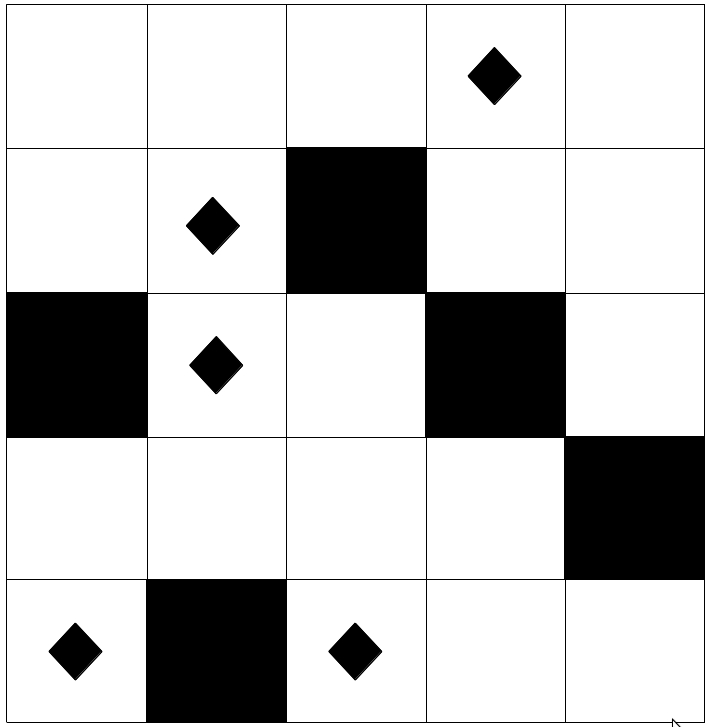
\epsfig{file=ejemplo2_ej3.jpg, scale=0.13} % primera imagen colocada a la izquierda
\caption{Ejemplo de la entrada de un caso sin solución.}
\end{center}
\label{fig-tc1}
\end{minipage}
\end{figure}
\end{center}

En el ejemplo de la Figura 14, se puede observar un caso que no tiene solución. Esto se debe a que la celda (5,1) contiene un casillero importante que debe ser atravesado por dos lásers simultáneamente. Dado que éste se encuentra en una esquina del tablero y posee una pared a su lado, no puede ser atravesado por un láser horizontal.

\textbf{Formato de entrada:} 
$$5\ \ 5$$
$$1\ \ 1\ \ 1\ \ 2\ \ 1$$
$$1\ \ 2\ \ 0\ \ 1\ \ 1$$
$$0\ \ 2\ \ 1\ \ 0\ \ 1$$
$$1\ \ 1\ \ 1\ \ 1\ \ 0$$
$$2\ \ 0\ \ 2\ \ 1\ \ 1$$
\textbf{Formato de salida:} $$-1$$\newline
\end{itemize}

\subsection{Resolución coloquial}

Para resolver el problema presentado decidimos utilizar la técnica de $backtracking$. Ésta consiste en evaluar las posibles combinaciones de soluciones del problema almacenándolas hasta llegar a la deseada. Para ello, definimos criterios de parada que nos permitieran decidir si las soluciones parcialmente obtenidas eran candidatas a soluciones válidas.\newline
\newline
Para lograr una correcta visualización del problema, representamos el piso entero del museo con una matriz, respetando las paredes y las casillas importantes. Luego, cada elemento de la matriz representa a una baldosa/casillero del piso y almacena el estado de la misma. Esto significa que de acuerdo a si contiene un 0, un 1 o un 2, podemos saber si hay algún sensor en ella o si le pasa algún láser por encima.\newline
\newline
Nuestro algoritmo, en primera instancia, genera un árbol de decisiones sobre todas las combinaciones posibles de cada casillero. Para lograrlo, recorre paulatinamente la matriz mencionada y, en cada paso, toma una decisión sobre el casillero actual para avanzar, luego, al siguiente. Las posibles decisiones son colocar o no algún sensor, empezando por intentar con el sensor cuatridireccional, para proseguir con el horizontal, luego el vertical y por último sin ningún sensor. Con el fin de acotar el tiempo de ejecución del algoritmo, se idearon ciertas cotas que frenan la ramificación del nodo que llega a algún caso que no tiene solución. Las cotas implementadas fueron las siguientes:
\begin{enumerate}
\item Una vez que se encuentra una solución, se almacena su costo y cualquier rama cuyo costo actual sea mayor al $almacenado-2000$ (siendo 2000 = diferencia entre un sensor cuatridireccional y uno bidireccional) es descartado.
\item Sobre las casillas importantes no puede haber ningún sensor cuatridireccional. Esto se debe a que en dicho caso, no existiría la posibilidad de atravesarlo por dos lásers sin que se rompan.
\item No puede haber ningún sensor vertical en las filas que tengan algún casillero importante, lo mismo para sensores horizontales en la columna. Esto se debe al mismo motivo mencionado en el ítem anterior.
\item Cualquier fila conteniendo algún sensor vertical no puede tener ninguno horizontal pues provocará un choque entre ellos. Análogamente de para una columna conteniendo un sensor horizontal a la que se le quiera agregar uno vertical.
\end{enumerate}
De este modo, el árbol realizado contiene en cada nodo una posibilidad de casillero y, como máximo, tres hermanos con las otras posibilidades. Luego, el árbol es recorrido y se comparan los precios de cada solución válida hasta llegar a una mínima.\newline
\newline

El pseudocódigo que describe la solución a nuestro problema es el siguiente:

\begin{algorithm}[H]
	\SetAlgoLined
	\caption{Algoritmo de Backtracking}
	\KwIn{Matriz $grilla$}
	\KwOut{Lista sensores}
	
	Matriz $mejorGrilla$
	Lista $casillasLibres$\\

	\For{Posicion $p \in grilla$}{
		\If{p esta libre}{
			$casillasLibres \leftarrow p$\\
		}
		\If{$p$ es importante}{
			\textbf{RestringirPorImportantes}(p)\\
		}
	}

	sensores := backtrack($grilla$, $casillasLibres$, $mejorGrilla$)\\

	\textbf{devolver} sensores
\end{algorithm}

\begin{algorithm}[H]
	\SetAlgoLined
	\caption{backtrack}
	\KwIn{Matriz $grilla$, Lista $casillasLibres$, Matriz $mejorGrilla$}
	\KwOut{Lista sensores}

    \If{$costoActual$ > $(mejorCostoObtenido - 2000)$}{
        backtrack($grilla$, $casillasLibres$)\\
	}
	
	\If{sensores esta vacio}{
		\If{chequearSolucion($grilla$) \land $ (costoActual $ < $ mejorCostoObtenido)$}{
			$mejorCostoObtenido$ := $costoActual$\\
			$mejorGrilla$ := $grilla$
		}
    }

	Casilla $casillaActual$ := Proxima casilla libre \in casillasLibres\\
	
	\If{$¬$sePuedeColocarUnSensor($casillaActual$)}{
		$mejorCostoObtenido$ := $costoActual$\\
		$mejorGrilla$ := $grilla$
	}
	
	\If{Puedo poner un sensor bidireccional en $casillaActual$}{
		Restringir por láser bidireccional\\
		Saco casillaActual de casillasLibres\\
		backtrack($grilla$, $casillasLibres$)\\
	}
	\If{Puedo poner un sensor vertical en $casillaActual$}{
		Restringir por láser vertical\\
		Restringir casilleros horizontales\\
		Saco casillaActual de casillasLibres\\
		backtrack($grilla$, $casillasLibres$)\\
	}
	\If{Puedo poner un sensor horizontal en $casillaActual$}{
		Restringir por láser horizontal\\
		Restringir casilleros verticales\\
		Saco casillaActual de casillasLibres\\
		backtrack($grilla$, $casillasLibres$)\\
	}

	Dejo el casillero en blanco\\
	backtrack($grilla$, $casillasLibres$)\\

	\textbf{devolver} ContarSensores($grilla$)
\end{algorithm}

\subsection{Demostración de correctitud}

Para demostrar la correctitud de nuestro algoritmo, debemos probar que se cumplen las siguientes propiedades:
\begin{itemize}
\item Nuestro algoritmo genera todas las combinaciones posibles para cada casillero.
\item Las podas utilizadas no alteran la solución final.
\item La solución es óptima, es decir, no existe otra cuyo costo sea menor.
\end{itemize}

\newline

\textbf{Nuestro algoritmo genera todas las combinaciones posibles para cada casillero.} \newline

Esto ocurre pues, para cada elemento de la matriz mencionada, se evalúan las cuatro posibilidades (sensor horizontal, sensor vertical, sensor cuatridimensional y sin sensor) sin tener en cuenta la decisión de la casilla anterior, siempre y cuando el caso no esté contemplado en alguna poda o no rompa los casos especificados en el enunciado. Luego, todas las combinaciones posibles de casos son generadas.\newline
\newline 

\textbf{Las podas utilizadas no alteran la solución final} \newline

Veamos que las podas elegidas no modifican la solución óptima:
\begin{itemize}
\item Poda nº1: Llamemos $T$ al costo de la mejor solución generada por el algoritmo en determinado momento. Si cualquier otra solución parcial ya alcanza el costo de $T$-2000 pueden ocurrir dos cosas: que el costo final de dicha solución sea $T$-2000 o que sea mayor a $T$. No existe otra opción pues 2000 es la diferencia en módulo que hay entre un sensor y el otro. Luego, esta poda descarta aquellas soluciones parciales cuyos costos superen los $T$-2000 asegurando no eliminar soluciones factibles.  
\item Poda nº2: Debido a que cualquier sensor cuatridimensional aplicado a una casilla importante rompe con los criterios que validan un piso, esta cota no elimina casos que pueden ser solución óptima.
\item Poda nº3: Cada casillero importante debe ser atravesado por dos sensores en simultáneo. Dado que este caso abarca la situación en la que hay un sensor horizontal en la columna de la casilla importante o vertical en su fila, no puede haber solución válida. Por lo tanto, se le quita la oportunidad de solución a dichas opciones, dándole a dicha restricción no sólo el atributo de poda, sino que también el de condición necesaria para que sea solución óptima.
\item Poda nº4: Al igual que en el caso anterior, aplicar un sensor bidimensional horizontal impide el agregado de sensores verticales en la misma columna y viceversa con las filas. Lo mismo ocurre con el agregado de sensores cuatridimensionales, que impiden la inserción de otro sensor en la misma fila o columna. Esta poda descarta soluciones inválidas sin alterar el resultado del problema.
\end{itemize}

\textbf{La solución es óptima, es decir, no existe otra cuyo costo sea menor.} \newline

Dado que nuestro algoritmo compara el valor de la solución creada con la más óptima almacenada y, en caso de que el costo de ésta última sea menor reemplaza la más óptima por ésta, el resultado final es la solución con menor costo de entre todas las posibles.


\subsection{Complejidad del algoritmo}

Dado que tenemos $n$x$m$ baldosas a partir de las que nuestro algoritmo genera 4 casos distintos para cada una de éstas, obtenemos $4^{nxm}$ combinaciones posibles. A su vez, por cada uno de estos casos se realizan una serie de operaciones, entre las cuales se encuentran:
\begin{itemize}
\item $Colocar\ sensores\ verticales$ y $Restringir\ celdas\ verticales$: Estas funciones en el peor de los casos recorren toda una columna de la matriz por lo que tienen complejidad $\mathcal{O}(n)$.
\item $Colocar\ sensores\ horizontales$ y $Restringir\ celdas\ horizontales$: Estas funciones en el peor de los casos recorren toda una fila de la matriz por lo que tienen complejidad $\mathcal{O}(m)$.
\item $Chequear\ solución$: Esta función recorre toda la matriz para corroborar si contiene una solución válida o no, luego su complejidad es de $\mathcal{O}(nxm)$.
\end{itemize}

En los casos en los que se coloca un sensor en una casilla libre, se pueden usan las funciones $Colocar$ $sensores$ $verticales$ $horizontales$ y $Restringir$ $celdas$ $horizontales/verticales$ o $Colocar$ $sensores$ $verticales$ y $Colocar$ $sensores$ $horizontales$. En ambos casos, éstas tienen complejidad $\mathcal{O}(n+m)$ ya que consiste en la suma de ambas complejidades debido a que las funciones se realizan paralelamente. Por otro lado, en gran parte de los nodos se verifica si la solución a la que se llegó resuelve o no el problema, por lo que el costo de cada nodo podría ser acotado por la complejidad de $chequear$ $solución$ ($mathcal{O}(nxm)$).\newline
\newline
A partir de lo mencionado precedentemente y teniendo en cuenta que tenemos $4^{nxm}$ combinaciones posibles cuyas complejidades son $\mathcal{O}(nxm)$ en el peor de los casos, nuestro algoritmo tiene un costo de $\mathcal{O}(n$x$m)$x$4^{n$x$m}$. Resulta importante mencionar que, si bien la complejidad del algoritmo no lo refleja, las podas cumplen un trabajo fundamental a la hora de medir la ejecución del algoritmo temporalmente. Esto se debe a que evitan que se generen todos los casos (tanto válidos como inválidos) reduciendo considerablemente el tiempo de ejecución del mismo en el caso promedio. Sin embargo, éstas pueden empeorar la complejidad del algoritmo dado que realizan operaciones 'extra' y en algunos casos pueden no ser utilizadas.

\subsection{Código fuente}

\begin{figure}[H]
\begin{center}
\begin{verbatim}
for (int i = 0; i < g.size(); ++i) {
   for (int j = 0; j < g[i].size(); ++j) {
      if (g[i][j].tipo == 2)
         restringirCasillasPorImportante(i, j); 
         if (g[i][j].tipo == 1) 
            casillasLibres.push(&(g[i][j]));
         }
      }
\end{verbatim}
\caption{Restringe las casillas según corresponde}
\end{center}
\end{figure}

\begin{figure}[H]
\begin{center}
\begin{verbatim}
if (casillasLibres.empty()) {
   if (chequearSolucion()) { 
      if (costoActual < mejorCosto) {
         haySolucion = true;
         mejorCosto = costoActual;
         gMejor = g;	
         mejorCantSensores = cantSensores;
        }
    }
    return;
}
\end{verbatim}
\caption{Condicional que almacena la mejor solución}
\end{center}
\end{figure}

\begin{figure}[H]
\begin{center}
\begin{verbatim}
if (costoActual > (mejorCosto-2000))
   return;
Casilla* casillaActual = casillasLibres.front();  
casillasLibres.pop();
if (casillaActual->laser > 0) {
   backtrack();
   casillasLibres.push(casillaActual);
   return;
} else {
   if (casillaActual->restricciones[2]){ 
      casillaActual->ocupado = true;
      casillaActual->tipoSensor = 1;
      casillaActual->laser = 3;
      laserVertical(casillaActual->i, casillaActual->j, "PONER");
      laserHorizontal(casillaActual->i, casillaActual->j, "PONER");
      costoActual = costoActual + 6000;
\end{verbatim}
\caption{Diferentes podas utilizadas}
\end{center}
\end{figure}

\begin{figure}[H]
\begin{center}
\begin{verbatim}
      cantSensores++;
      backtrack();
      cantSensores--;
      costoActual = costoActual - 6000;
      laserVertical(casillaActual->i, casillaActual->j, "SACAR");
      laserHorizontal(casillaActual->i, casillaActual->j, "SACAR");
}
if (casillaActual->restricciones[0]){ 
      casillaActual->ocupado = true;
      casillaActual->tipoSensor = 2;
      casillaActual->laser = 1;
      vector< vector <int> >cache;
      for (int i = 0; i < g.size(); ++i)
      cache.push_back(g[i][casillaActual->j].restricciones);
      restringVertical(casillaActual->i, casillaActual->j);
      laserHorizontal(casillaActual->i, casillaActual->j, "PONER");
      costoActual = costoActual + 4000;
      cantSensores++;
      backtrack();
      cantSensores--;
      costoActual = costoActual - 4000;
      laserHorizontal(casillaActual->i, casillaActual->j, "SACAR");
      for (int i = 0; i < cache.size(); ++i)
         g[i][casillaActual->j].restricciones = cache[i];
}
if (casillaActual->restricciones[1]){ 
      casillaActual->ocupado = true;
      casillaActual->tipoSensor = 3;
      casillaActual->laser = 2;
      vector< vector <int> >cache;			
      for (int i = 0; i < g[casillaActual->i].size(); ++i)
         cache.push_back(g[casillaActual->i][i].restricciones);
      restringHorizontal(casillaActual->i, casillaActual->j);
      laserVertical(casillaActual->i, casillaActual->j, "PONER"); 
      costoActual = costoActual + 4000;
      cantSensores++;
      backtrack();
      cantSensores--;
      costoActual = costoActual - 4000;
      laserVertical(casillaActual->i, casillaActual->j, "SACAR");
      for (int i = 0; i < cache.size(); ++i)
         g[casillaActual->i][i].restricciones = cache[i];
}
casillaActual->ocupado = false;
casillaActual->tipoSensor = -1;
casillaActual->laser = 0;	
backtrack();
casillasLibres.push(casillaActual);
return;

\end{verbatim}
\caption{Diferentes podas utilizadas}
\end{center}
\end{figure}



\subsection{Instancias posibles}
Para verificar la correctitud de nuestro programa, dispusimos variar estratégicamente las instancias de entrada al ejecutarlo.
\begin{itemize}
\item En primer lugar, ejecutamos el programa ingresando una única casilla libre, siendo ésta un lugar importante. Dicha prueba se realizó con el fin de verificar que nuestro algoritmo devolviera $-1$ dado que no existe la posibilidad de insertar 2 lásers en ese espacio, siendo este el requisito para los espacios importantes.\newline

\textbf{Parámetro de entrada:} 
$$3\ \ 3$$
$$0\ \ 0\ \ 0$$
$$0\ \ 2\ \ 0$$
$$0\ \ 0\ \ 0$$
\textbf{Parámetro de salida:} $$-1$$\newline

\begin{center}
\begin{figure}[H] % indico que voy a poner una figura y [h] indica que la posición relativa, tambien puedo usar t = top entre otros.
\begin{minipage}[t]{.45\textwidth}
\begin{center}

\epsfig{file=instanciaposible_ej3_in1.jpg, scale=0.13} % primera imagen colocada a la izquierda
\caption{Entrada de la instancia posible Nº1.}
\end{center}
\label{fig-tc1}
\end{minipage}
\end{figure}
\item Por otra parte, probamos el programa para un museo conformado únicamente por paredes, en otras palabras, el caso vacío. Lo relevante de este caso es que nuestro algoritmo lo considera y otorga, como salida, que la solución es no colocar ningún láser.\newline
\end{center}

\textbf{Parámetro de entrada:} 
$$3\ \ 3$$
$$0\ \ 0\ \ 0$$
$$0\ \ 0\ \ 0$$
$$0\ \ 0\ \ 0$$
\textbf{Parámetro de salida:} $$0\ \ 0$$\newline
\item Otro caso interesante es analizar la solución obtenida al tener todos espacios libres. La idea de dicho caso consiste en comprobar que el algoritmo devuelve la solución más económica del problema.\newline

\textbf{Parámetro de entrada:} 
$$3\ \ 3$$
$$1\ \ 1\ \ 1$$
$$1\ \ 1\ \ 1$$
$$1\ \ 1\ \ 1$$
\textbf{Parámetro de salida:} 
$$3\ \ 12000$$
$$2\ \ 0\ \ 0$$
$$2\ \ 1\ \ 2$$
$$2\ \ 2\ \ 0$$
\newline

\begin{figure}[H] % indico que voy a poner una figura y [h] indica que la posición relativa, tambien puedo usar t = top entre otros.
\hfill
\begin{minipage}[t]{.45\textwidth}
\begin{center}

\epsfig{file=instanciaposible_ej3_in3.jpg, scale=0.15} % primera imagen colocada a la izquierda
\caption{Entrada de la instancia posible Nº3.}
\label{fig-tc1}
\end{center}
\end{minipage}
\hfill
\begin{minipage}[t]{.45\textwidth}
\begin{center}
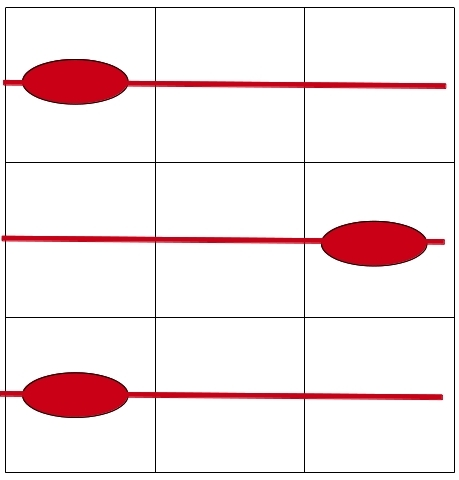
\epsfig{file=instanciaposible_ej3_out3.jpg, scale=0.15} % segunda imagen colocada a la derecha
\caption{Salida de la instancia posible Nº3.}
\label{fig-tc2}
\end{center}
\end{minipage}
\hfill
\end{figure}

\item Por otra parte, resulta importante corroborar la solución en el caso en el que todos los espacios son importantes. En este caso particular no existe solución ya que no podrían pasar dos lásers por el mismo casillero especial sin que uno de estos toque a otro láser.\newline

\textbf{Parámetro de entrada:} 
$$3\ \ 3$$
$$2\ \ 2\ \ 2$$
$$2\ \ 2\ \ 2$$
$$2\ \ 2\ \ 2$$
\textbf{Parámetro de salida:} $$-1$$\newline

\begin{center}
\begin{figure}[H] % indico que voy a poner una figura y [h] indica que la posición relativa, tambien puedo usar t = top entre otros.
\begin{minipage}[t]{.45\textwidth}
\begin{center}
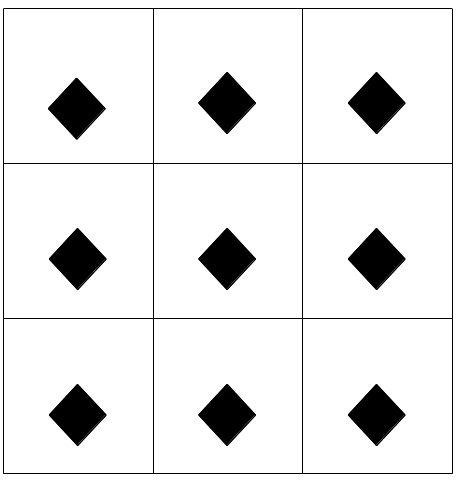
\epsfig{file=instanciaposible_ej3_in4.jpg, scale=0.13} % primera imagen colocada a la izquierda
\caption{Entrada de la instancia posible Nº4.}
\end{center}
\label{fig-tc1}
\end{minipage}
\end{figure}
\item Por otra parte, probamos el programa para un museo conformado únicamente por paredes, en otras palabras, el caso vacío. Lo relevante de este caso es que nuestro algoritmo lo considera y otorga, como salida, que la solución es no colocar ningún láser.\newline
\end{center}

\item Otra situación posible es en la que se encuentran alternados los casilleros de piso y pared. De este caso puede destacarse que no es posible aplicar ninguna de las podas mencionadas.\newline
\textbf{Parámetro de entrada:} 
$$3\ \ 3$$
$$1\ \ 0\ \ 1$$
$$0\ \ 1\ \ 0$$
$$1\ \ 0\ \ 1$$
\textbf{Parámetro de salida:} 
$$5\ \ 20000$$
$$2\ \ 0\ \ 0$$
$$2\ \ 0\ \ 2$$
$$2\ \ 1\ \ 1$$
$$2\ \ 2\ \ 0$$
$$2\ \ 2\ \ 2$$

\begin{figure}[H] % indico que voy a poner una figura y [h] indica que la posición relativa, tambien puedo usar t = top entre otros.
\hfill
\begin{minipage}[t]{.45\textwidth}
\begin{center}
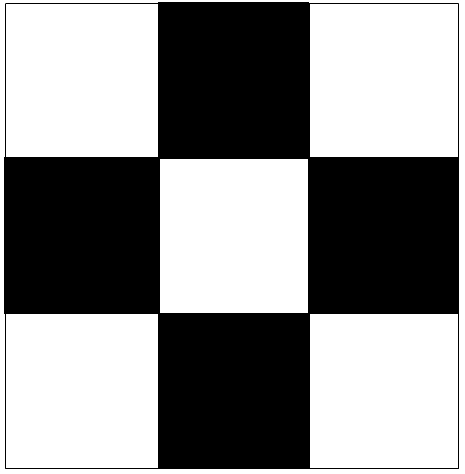
\epsfig{file=instanciaposible_ej3_in5.jpg, scale=0.15} % primera imagen colocada a la izquierda
\caption{Entrada de la instancia posible Nº5.}
\label{fig-tc1}
\end{center}
\end{minipage}
\hfill
\begin{minipage}[t]{.45\textwidth}
\begin{center}
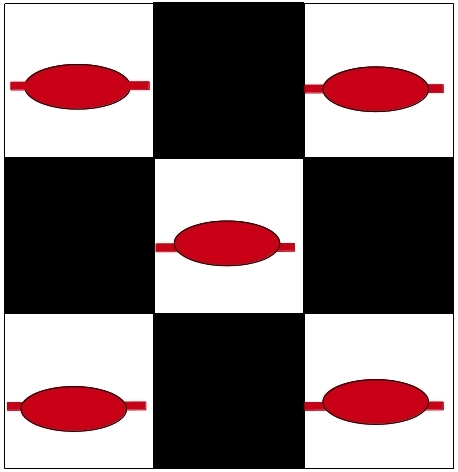
\epsfig{file=instanciaposible_ej3_out5.jpg, scale=0.15} % segunda imagen colocada a la derecha
\caption{Salida de la instancia posible Nº5.}
\label{fig-tc2}
\end{center}
\end{minipage}
\hfill
\end{figure}

\item Por último, se encuentra el caso en el que coexisten los 3 tipos de casilleros, siendo éste el mas típico del problema. \newline

\textbf{Parámetro de entrada:} 
$$3\ \ 3$$
$$1\ \ 1\ \ 1$$
$$1\ \ 2\ \ 0$$
$$0\ \ 0\ \ 1$$
\textbf{Parámetro de salida:} 
$$3\ \ 14000$$
$$1\ \ 0\ \ 1$$
$$2\ \ 1\ \ 0$$
$$2\ \ 2\ \ 2$$
\newline
\end{itemize}

\begin{figure}[H] % indico que voy a poner una figura y [h] indica que la posición relativa, tambien puedo usar t = top entre otros.
\hfill
\begin{minipage}[t]{.45\textwidth}
\begin{center}
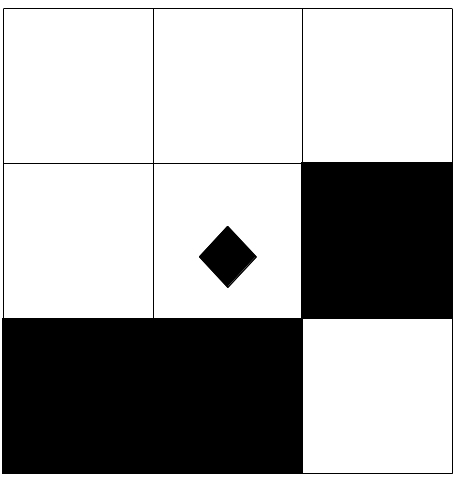
\epsfig{file=instanciaposible_ej3_in6.jpg, scale=0.15} % primera imagen colocada a la izquierda
\caption{Entrada de la instancia posible Nº6.}
\label{fig-tc1}
\end{center}
\end{minipage}
\hfill
\begin{minipage}[t]{.45\textwidth}
\begin{center}
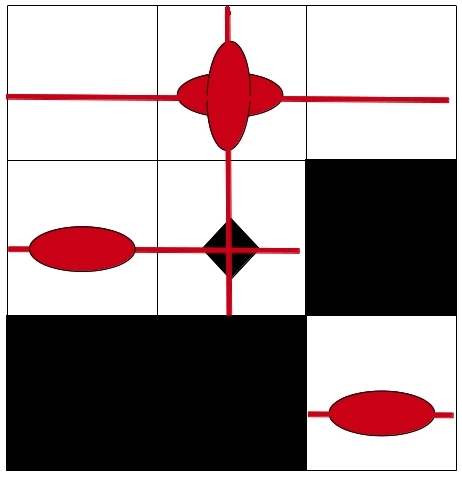
\epsfig{file=instanciaposible_ej3_out6.jpg, scale=0.15} % segunda imagen colocada a la derecha
\caption{Salida de la instancia posible Nº6.}
\label{fig-tc2}
\end{center}
\end{minipage}
\hfill
\end{figure}

\subsection{Testing}
Para las pruebas de testing, hicimos diferentes instancias que nos permitieran poner a prueba varias caracteristicas de nuestro algoritmo, como la calidad de las podas y que tanto mejoran los tiempos de la ejecución cuando éstas son aplicadas con mayor frecuencia, tambien buscamos instancias que nos permitieran medir los tiempos de ejecución tratando de minimizar la efectividad de las podas y por ultimo hicimos un test aleatorio para poder ver el funcionamiento general del algoritmo.

Para los test aleatorios tomamos valores de configuracion que limitan algunas caracteristicas de estos con el fin de evitar casos en donde el algoritmo de incorrecto rápidamente o que dada la cantidad de paredes dentro de la matriz el problema sea reducido a una instancia de menor tamaño. Para evitar esto decidimos que la cantidad de paredes iba a ser el 20\% del total de la cantidad de casilleros y que la cantidad de lugares importantes iba a ser el 10\%, elegimos estos valores para mantener el tamaño de los casilleros libres lo suficientemente grande para que no se iguale al tamaño de una instancia menor. Para generar estos casos basicamente lo quehicimos fue crear un vector de n*m posiciones donde cada posicion tiene un 1 (piso) por defecto y luego tomar el 20\% de ese vector y ponerlo en 0 (pared) y luego tomar otro 10\% que no sea pared y ponerlo en 2 (importante), luego utilizamos la funcion \textbf{shuffle} para mezclar de forma aleatoria el array y lo escribimos en pantalla respetando el formato de entrada del ejercicio.

Trataremos de mostrar que los tiempos de ejecución de aproximan a la complejidad que calculamos que es $O((n*m)*4^{n*m})$ y que en ciertos casos, a pesar que las podas bajen los tiempos de ejecucion, por las caracteristicas de las instancias igual se puede ver que la funcion crece asintoticamente aproximandose a la cota de complejidad dada.

Las funciones de complejidad fueron aproximadas a los datos de complejidad de cada conjunto de instancias por algoritmos matematicos en donde se modifican constantes multiplicativas y aditivas de forma tal que la funcion resultante este lo mas cerca posible de los tiempos dados por los resultados.

El tamaño de entrada en todos los casos esta definido en funcion de la cantidad de casilleros, donde $n$ es el ancho de la matriz que representa la entrada y $m$ es el alto.

Los tiempos estan dados en nanosegundos, decidimos no hacer reducciones de los valores de entrada por que estos estaban entre los rangos de $1^{3}$ y $1^{11}$ y nos parecio importante mostrar que eventualmente en casos que no difieren mucho de su tamaño de instancia, el tiempo de ejecucion si disparaba.

\begin{figure}[H] %[h] Aqui [b] para button [t] para top
\begin{center}
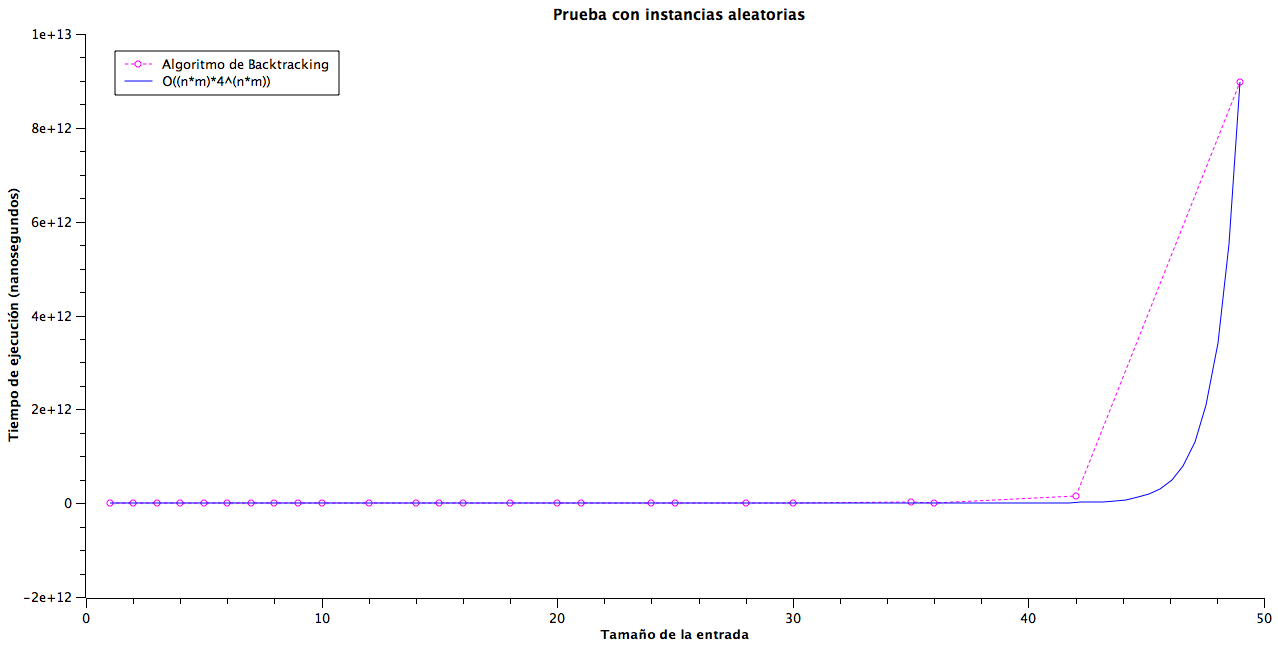
\includegraphics[width=460pt]{../imgs/graficoej3_aleatorio.png}
\end{center}
\caption{Prueba con instancias aleatorias}
\end{figure}

En este caso vemos como efectivamente la funcion crece aproximandose a la complejidad que definimos. Estos casos aleatorios estan definidos en funcion tableros cuya cantidad de elementos esta compuesta por un 20\% paredes, 10\% casilleros importantes y 70\% casilleros comunes. este grafico posee datos de varias ejecuciones del algoritmo con diferentes entradas aleatorias con iguales pocentajes y diferente distribucion que luego se promediaron para asi minimizar casos particulares en donde por diversos motivos (como las podas) la ejecucion termine mucho antes.


\begin{figure}[H] %[h] Aqui [b] para button [t] para top
\begin{center}
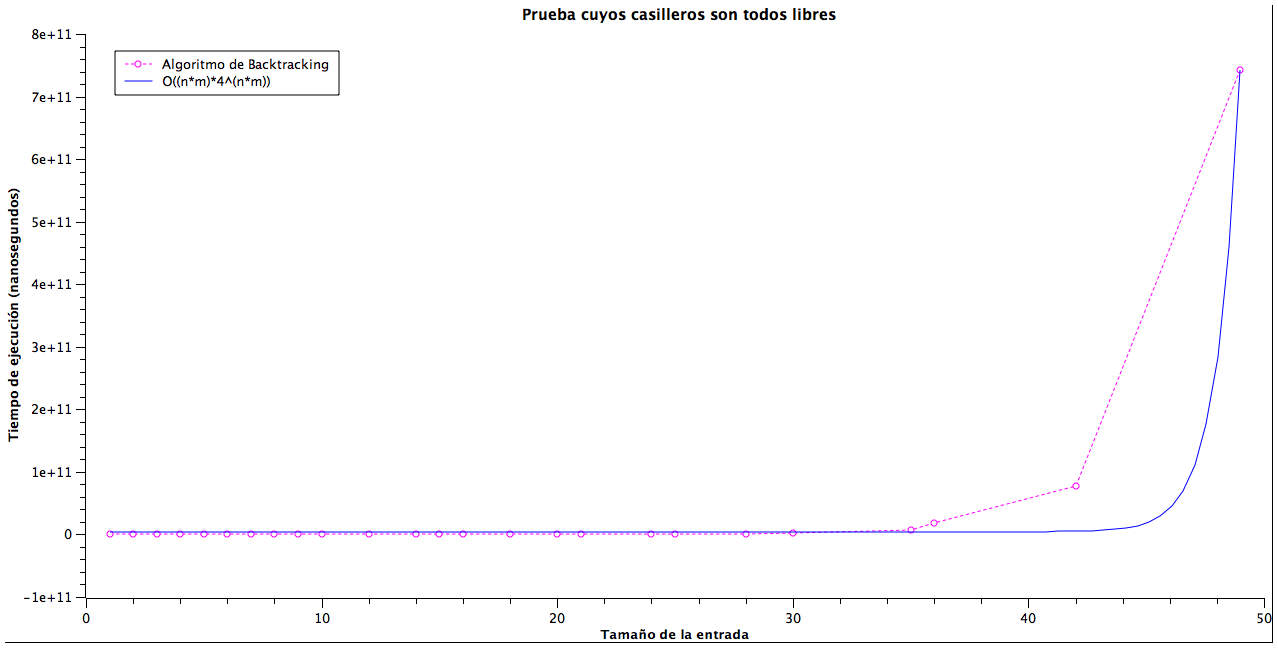
\includegraphics[width=460pt]{../imgs/graficoej3_todosUno.png}
\end{center}
\end{figure}

En este caso intentamos generar instancias que tuvieran todos los casilleros como espacios libres, sin paredes ni lugares importantes, para maximizar la cantidad de casilleros que puede intentar usar el algoritmo para probar combinaciones, los tiempos de esta corrida son en general bajos ya que las podas hacen un gran trabajo reduciendo la cantidad de opciones en cada paso ya por cada sensor que ponga la cantidad de casillas que voy a cubrir va a ser de al menos todo el ancho o el alto del tablero debido a que no hay paredes que lo detengan.

\begin{figure}[H] %[h] Aqui [b] para button [t] para top
\begin{center}
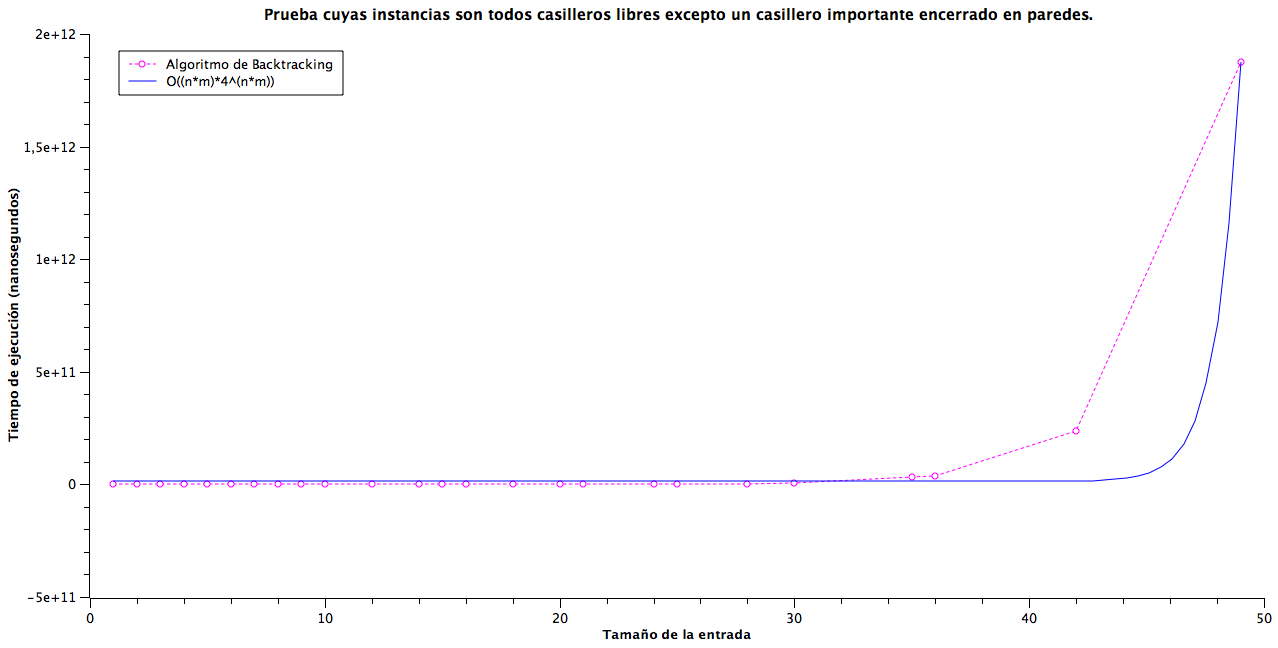
\includegraphics[width=460pt]{../imgs/graficoej3_todosUnoSinSolucion.png}
\end{center}
\end{figure}

En este caso hicimos lo mismo que antes, solo que forzamos una combinacion de paredes y casilleros importantes que provoca que el algoritmo no encuentre ninguna solucion, y de hecho, no haya ninguna solucion al tablero en cuestion, de esta  manera nos evitamos que enrte en juego una de las podas mas improtantes, que es la que guarda el costo de una solucion y nunca busca soluciones cuyo costo sea mayor al actual, como en ningun momento encontramos ninguna solucion, nunca actualizamos ese costo de la solucion entonces el algoritmo va a seguir intentando todas las posibles combinaciones hasta que concluya que no hay ninguna combinacion posible para resolver el tablero, sin embargo las podas que se producen al colocar un laser siguen hacienod que se resuelve un poco mas rapido.

\begin{figure}[H] %[h] Aqui [b] para button [t] para top
\begin{center}
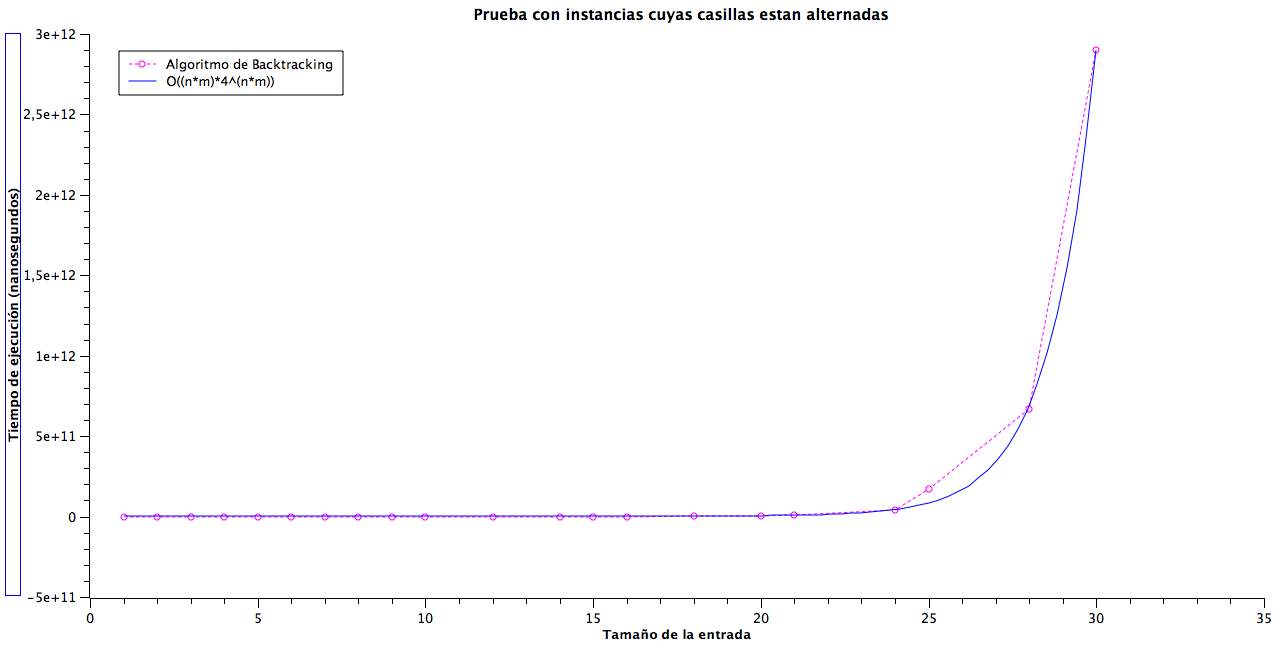
\includegraphics[width=460pt]{../imgs/graficoej3_alternado.png}
\end{center}
\end{figure}

Este es un caso que encontramos que tiene la particularidad de anular casi todas las podas que pensamos para el ejercicio, la forma de este caso tiene el formato de la Figura 23 y es una generalizacion del mismo para tamaños de n*m. Por el orden en el cual nuestro algirmto intenta poner los sensores (primero los mas caros y luego los mas baratos) éste tarda mucho en encontrar la solucion correcta y su tiempo de ejecucion se extendio tanto que no pudimos llegar a correr los tamaños de test que corrimos para los otros ejemplos. Este caso 

